% Gemini theme
% Author: Ranji Raj
% A fork of https://github.com/ranjiGT/

\documentclass[final]{beamer}

% ====================
% Packages
% ====================

\usepackage[T1]{fontenc}
\usepackage{lmodern}
\usepackage[size=custom,width=120,height=72,scale=1.0]{beamerposter}
\usetheme{gemini}
\usecolortheme{uchicago}
\usepackage{graphicx}
\usepackage{booktabs}
\usepackage{tikz}
\usepackage{fontawesome5}
\usepackage{pgfplots}
\pgfplotsset{compat=1.17}

% ====================
% Lengths
% ====================

% If you have N columns, choose \sepwidth and \colwidth such that
% (N+1)*\sepwidth + N*\colwidth = \paperwidth
\newlength{\sepwidth}
\newlength{\colwidth}
\setlength{\sepwidth}{0.025\paperwidth}
\setlength{\colwidth}{0.3\paperwidth}

\newcommand{\separatorcolumn}{\begin{column}{\sepwidth}\end{column}}

% ====================
% Title
% ====================

\title{Object detection using Semi-Supervised Classification}

\author{Shubham Kumar Agrawal \inst{1} \and Pavan Tummala \inst{1} \and Usama Ashfaq \inst{1} \and Ranjiraj Rajendran Nair \inst{2} \and Syed Muhammad Laique Abbas \inst{2}}

\institute[shortinst]{\inst{1} Faculty of Computer Science: Digital Engineering \samelineand \inst{2} Faculty of Computer Science: Data and Knowledge Engineering}

% ====================
% Footer (optional)
% ====================

\footercontent{
  \href{https://github.com/ranjiGT/}{\raisebox{-0.2\height}\faGithub\ \underline{github.com/ranjiGT}} \hfill
  Advanced Topics in Machine Learning --- Summer 2021 \hfill
  Group: T02}
% (can be left out to remove footer)

% ====================
% Logo (optional)
% ====================

% use this to include logos on the left and/or right side of the header:
% \logoright{
\includegraphics[height=7cm]{logos/ovgu.pdf}}
 %\logoleft{\includegraphics[height=7cm]{logo2.pdf}}

% ====================
% Body
% ====================

\begin{document}
\addtobeamertemplate{headline}{}
{
    \begin{tikzpicture}[remember picture,overlay]
      \node [anchor=north west, inner sep=3cm] at ([xshift=0.0cm,yshift=1.0cm]current page.north west)
      {
\includegraphics[height=5.0cm]{logos/OvGU-Logo_schwarz.eps}}; % also try shield-white.eps
      %\node [anchor=north east, inner sep=3cm] at %([xshift=0.0cm,yshift=2.5cm]current page.north east)
      %{\includegraphics[height=5.0cm]{}};
    \end{tikzpicture}
}

\begin{frame}[t]
\begin{columns}[t]
\separatorcolumn

\begin{column}{\colwidth}

  \begin{block}{Motivation and Problem Statement}
  
    \textbf{Motivation}: The Proceedings of the European Conference on Computer Vision has conducted a benchmark PASCAL Visual Object Challenge (VOC) evaluating performance on object class recognition (from 2005-2012, now finished). For our task, we examine the 2007 dataset which consists of several types of random images collected in January 2007 from \textit{Flickr}. There are five challenges: classification, detection, segmentation, action classification, and person layout. 
    
    \textbf{Problem Statement}: Our goal from this challenge is to perform \textbf{image classification} from several visual object classes in realistic scenes (i.e. not pre-segmented objects). And so, we will be using certain Semi-Supervised Learning approaches where we have both labeled and unlabeled sets to check if we get superior results as opposed to supervised techniques.
  \end{block}

  \begin{block}{Data set}
  
    The PASCAL Visual Object Classes Challenge (VOC 2007) data set consists of about 5,011 RGB images and 20 classes. The twenty object classes that have been selected are:

    \begin{itemize}
      \item \textbf{Person}: person
      \item \textbf{Animal}: bird, cat, cow, dog, horse, sheep
      \item \textbf{Vehicle}: aeroplane, bicycle, boat, bus, car, motorbike, train
      \item \textbf{Indoor}: bottle, chair, dining table, potted plant, sofa, tv/monitor
    \end{itemize}
    We represent the images in an array with their labels. The labeled set is partitioned into various split points ranging from [0.1,0.9] for our SSL strategy.
    
    \begin{figure}[ht]
    \begin{minipage}[b]{.40\textwidth}
    \centering
    \includegraphics[width=9cm, height=9cm]{pca.jpg}
    \caption{Feature space by PCA}
    \label{fig:pca}
    \end{minipage}\qquad
    \begin{minipage}[b]{.40\textwidth}
    \centering
    \includegraphics[width=9cm, height=9cm]{tsne.png}
    \caption{Feature space by t-SNE}
    \label{fig:tsne}
    \end{minipage}
    \end{figure} 

  \end{block}

  \begin{alertblock}{SSL Concept}

    The SSL methods we proposed for solving our task as follows:
    \begin{itemize}
        \item (\textit{Graph-based}) \textbf{Label Propagation Algorithm (LPA)}: \textit{Assumption} - Similar images would have similar feature descriptors and so they would be mapped closely in the graph with high weights to the edges connecting to them.
        \item (\textit{Graph-based}) \textbf{Label Spreading Algorithm}:  \textit{Manifold Assumption} - the graphs, constructed based on the local similarity between features, provide a lower-dimensional representation of the high-dimensional input images (images on the same low-dimensional manifold should have the same label).
        \item (\textit{Inductive}) \textbf{Semi-Supervised Gaussian Mixture Model (SSGMM)}: \textit{Assumption} - The images come from the mixture model, where the number of features, prior $p(y)$, and conditional $p(x|y)$ are all correct.
    \end{itemize}

    
    \textbf{Advantages}: It highly reduces the amount of annotated data used for our task.\newline
    \textbf{Disadvantages}: Since all stated models of ours use an iterative approach for updating it can converge to local minima leading to less stable results.
    

  \end{alertblock}

\end{column}

\separatorcolumn

\begin{column}{\colwidth}

  \begin{block}{Implementation}
    For our task we used \textbf{Python 3+} for implementing our concepts. The open tool-kits that we used for our development purposes are primarily \textit{\textbf{Jupyter Notebook}} and \textit{\textbf{Spyder IDE}} from the \textbf{\textit{Anaconda}} distribution software. The list of the necessary libraries/packages used  has been made available in the \textit{requirements.txt} file. 

    We implemented a \textit{\textbf{Data Loader}} pipeline where we feed the images in an array along with their labels which goes for train-test-validate partition. We extracted the 3 mandatory features: \textit{MPEG-7 Color Layout Descriptor, Visual Bag-of-Words, \textbf{S}peeded \textbf{U}p \textbf{R}obust \textbf{F}eatures}. For the first feature, the process comprised of 4 phases namely: \textit{Image partitioning, Representative color selection, DCT transformation, Zigzag scanning}. For the second and third features combined, we extracted the features for each of the images using the functionalities provided by python \textit{OpenCV} library. Furthermore, we constructed a codebook vector using the \textit{k}-means clustering algorithm of a certain vocabulary size using the extracted features. For each feature, we assign a code from the codebook, and then produce a histogram for it, which we used as a feature to the model. For the extra  feature, we have the \textit{Local Binary Patterns} and \textit{Color Histogram}.
    
    \begin{figure}[ht]
    \begin{minipage}[b]{.40\textwidth}
    \centering
    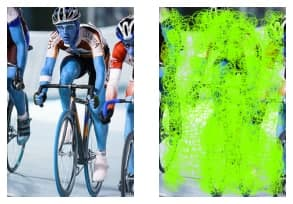
\includegraphics[width=9cm, height=4cm]{surf-1.jpg}
    %\caption{Feature space by PCA}
    \label{fig:keyp-1}
    \end{minipage}\qquad
    \begin{minipage}[b]{.40\textwidth}
    \centering
    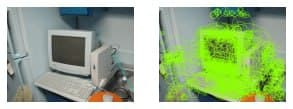
\includegraphics[width=9cm, height=4cm]{surf-2.jpg}
    %\caption{Feature space by t-SNE}
    \label{fig:keyp-2}
    \end{minipage}
    \caption{SURF key point visualization for images}
    \end{figure} 

    %\begin{enumerate}
     % \item \textbf{Label Propagation}, with safe SSL.
      %\item \textbf{Label Spreading}, with safe SSL.
      %\item \textbf{Semi-Supervised GMM}, with safe SSL.
    %\end{enumerate}

  \end{block}

  \begin{block}{Evaluation}
    \heading{Model selection}
    On the features we perform class balancing (\textit{undersampling}), feature selection (\textit{ANOVA}), feature reduction (\textit{PCA}) with an enumeration of \textbf{$2^c$} (where c is the total extracted features). Based on this, we analyze from a line plot for all the split points ranging from [0.1,0.9] which combination is better to be used for model building. After this process, we effectively depict a box plot to pick the best model. We are testing for 70 iterations. 
  \end{block}

  \begin{block}{Learning curves and Box plots}

    \begin{figure}[ht]
    \begin{minipage}[b]{.40\textwidth}
    \centering
    \includegraphics[width=12cm, height=10cm]{feat-seelct-LPA.jpg}
    \caption{Selecting the best feature}
    \label{fig:box-whisker-plot}
    \end{minipage}\qquad
    \begin{minipage}[b]{.40\textwidth}
    \centering
    \includegraphics[width=12cm, height=10cm]{boxplot_LPA.jpg}
    \caption{Box plot for \textit{Label Propagation}}
    \label{fig:lineplot-lpa}
    \end{minipage}
    %\caption{SURF key point visualization for images}
    \end{figure} 

    \begin{itemize}
        \item \textbf{Figure 4.} Proves a hypothesis that for all enumeration with a \textbf{two}-feature combination the "pink" curve outperforms others for all splits.
        \item \textbf{Figure 5.} Shows LPA run on \textit{stand-alone class balancing, class balancing with ANOVA, class balancing with PCA}. Here we state that \textit{class balancing with ANOVA} is superior in comparison to other models.  
    \end{itemize} 

    %\begin{itemize}
     % \item \textbf{Sed consequat} id ante vel efficitur. Praesent congue massa
      %  sed est scelerisque, elementum mollis augue iaculis.
       % \begin{itemize}
        %  \item In sed est finibus, vulputate
         %   nunc gravida, pulvinar lorem. In maximus nunc dolor, sed auctor eros
          %  porttitor quis.
          %\item Fusce ornare dignissim nisi. Nam sit amet risus vel lacus
          %  tempor tincidunt eu a arcu.
          %\item Donec rhoncus vestibulum erat, quis aliquam leo
           % gravida egestas.
        %\end{itemize}
      %\item \textbf{Sed luctus, elit sit amet} dictum maximus, diam dolor
       % faucibus purus, sed lobortis justo erat id turpis.
      %\item \textbf{Pellentesque facilisis dolor in leo} bibendum congue.
       % Maecenas congue finibus justo, vitae eleifend urna facilisis at.
    %\end{itemize}

  \end{block}

\end{column}

\separatorcolumn

\begin{column}{\colwidth}

  \begin{block}{Bar plots and ROC curves}

    \begin{figure}[ht]
    \begin{minipage}[b]{.40\textwidth}
    \centering
    \includegraphics[width=12cm, height=10cm]{Label_spreading_CPE.jpg}
    \caption{\textit{Label Spreading}-Prediction error}
    \label{fig:label-spreading-CPE}
    \end{minipage}\qquad
    \begin{minipage}[b]{.40\textwidth}
    \centering
    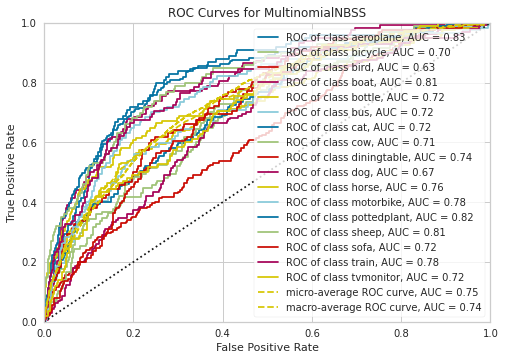
\includegraphics[width=12cm, height=10cm]{ROC-MNBSS_CB.png}
    \caption{ROC curve for \textit{SSGMM}}
    \label{fig:roc-SSGMM}
    \end{minipage}
    %\caption{SURF key point visualization for images}
    \end{figure} 

    \begin{itemize}
        \item \textbf{Figure 6.} Shows the support for 20 classes each fitted in  classification model which is displayed as a stacked bar for the \textit{Label Spreading} algorithm. 
        \item \textbf{Figure 7.} Depicts TPR vs. FPR for a non-decreasing ROC curve for 20 multiple classes with selective AUC values.  
    \end{itemize} 

    %\heading{A heading inside a block}

    %Praesent consectetur mi $x^2 + y^2$ metus, nec vestibulum justo viverra
    %nec. Proin eget nulla pretium, egestas magna aliquam, mollis neque. Vivamus
    %dictum $\mathbf{u}^\intercal\mathbf{v}$ sagittis odio, vel porta erat
    %$congue sed. Maecenas ut dolor quis arcu auctor porttitor.

    %\heading{Another heading inside a block}

    %Sed augue erat, scelerisque a purus ultricies, placerat porttitor neque.
    %Donec $P(y \mid x)$ fermentum consectetur $\nabla_x P(y \mid x)$ sapien
    %sagittis egestas. Duis eget leo euismod nunc viverra imperdiet nec id
    %justo.

  \end{block}

  \begin{block}{Conclusion}

    Upon the box plot realization from all the models, we conclude that the winner model can be declared as \textbf{Label Propagation} and \textbf{Label Spreading} with roughly 33\% accuracy. 

    \begin{table}
      \centering
      \begin{tabular}{l r r c}
        \toprule
        \textbf{Algorithms} & \textbf{Undersampling} & \textbf{Undersampling+ANOVA} & \textbf{Undersampling+PCA} \\
        \midrule
        Label Propagation & 28\% & \textbf{33\%} & 17\% \\
        Label Spreading & 28\% & \textbf{33\%} & 17\% \\
        SSGMM & 20.2\% & 19\% & 21.5\% \\
        %Qux & 7.59 & 974 & $\gamma$ \\
        \bottomrule
      \end{tabular}
      \caption{An overview of the results of our SSL techniques.}
    \end{table}

    It can be inferred that the transductive graph-based SSL approach showcased a better performance over the inductive technique for our task. We also ran a  "Safe SSL" check on the SSGMM where we used the stand-alone labeled set to run the supervised classifier and evaluate the performance of this on the test set. Moreover, we used the labeled set in conjunction with the unlabeled set to run the semi-supervised model and use it to evaluate the accuracy of this model on the test set. We can benchmark our models effectively for our task with these state-of-the-art SSL techniques to be devised as a baseline for future research in this field of interest.

     A similar proof of concept could be carried out with the \textbf{Active Learning} state-of-the-art algorithms and methods which utilize certain statistical theories to boost the predictive power of the model or with \textbf{online-SSL} where labeled and unlabeled instances arrive sequentially.
    
    \heading{Future work}
    \begin{itemize}
        \item \textbf{Model ensemble}: Combining classifiers by voting or averaging to improve performance.
        \item \textbf{Feature refining}: Add other relevant features for better results.
    \end{itemize}

  \end{block}

  \begin{block}{References}

    \nocite{*}
    \footnotesize{\bibliographystyle{plain}\bibliography{poster}}

  \end{block}

\end{column}

\separatorcolumn
\end{columns}
\end{frame}

\end{document}
